% Shared standalone design for the editable figure reconstructions.
\documentclass[tikz,border=5pt,10pt]{standalone}
\usepackage[T1]{fontenc}
\usepackage[utf8]{inputenc}
\usepackage{newpxtext,newpxmath}
\usepackage[scaled=.94]{sourcesanspro}
\usepackage{pgfplots}
\pgfplotsset{compat=1.18}
\usetikzlibrary{arrows.meta,calc,positioning,decorations.pathreplacing,
  decorations.markings,patterns,matrix,shapes.geometric,fit,backgrounds,
  intersections,angles,quotes}
\definecolor{ink}{HTML}{203746}
\definecolor{accent}{HTML}{146C78}
\definecolor{muted}{HTML}{667780}
\definecolor{signalred}{HTML}{B94B44}
\color{ink}
\tikzset{>=Latex,line width=.8pt,
  every node/.style={font=\small},
  axis/.style={->,draw=muted,line width=.5pt},
  guide/.style={draw=muted,dashed,line width=.45pt},
  curve/.style={draw=accent,line width=1pt},
  marker/.style={circle,fill=accent,inner sep=1.5pt},
  labelbox/.style={fill=white,inner sep=2pt}}

\begin{document}
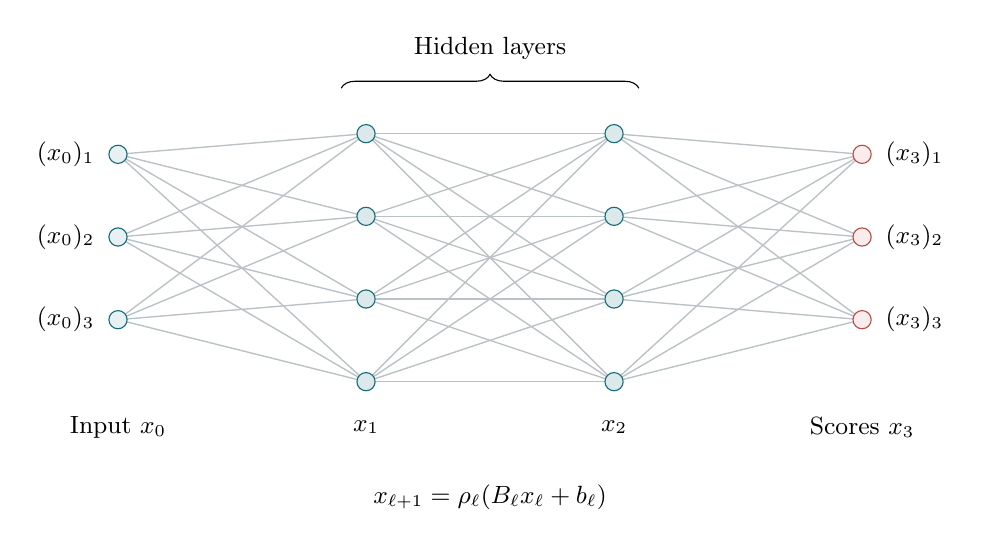
\begin{tikzpicture}[x=1.05cm,y=1.05cm]
\foreach \i in {1,2,3}{\coordinate(in\i)at(0,{4.5-\i});\coordinate(out\i)at(9,{4.5-\i});}
\foreach \i in {1,...,4}{\coordinate(a\i)at(3,{4.75-\i});\coordinate(b\i)at(6,{4.75-\i});}
\foreach \i in {1,2,3}{\foreach \j in {1,...,4}{\draw[muted!45,line width=.5pt](in\i)--(a\j);\draw[muted!45,line width=.5pt](b\j)--(out\i);}}
\foreach \i in {1,...,4}{\foreach \j in {1,...,4}{\draw[muted!45,line width=.5pt](a\i)--(b\j);}}
\foreach \i in {1,2,3}{\filldraw[draw=accent,fill=accent!10](in\i)circle(.11);\node[left=5pt]at(in\i){$(x_0)_{\i}$};\filldraw[draw=signalred,fill=signalred!10](out\i)circle(.11);\node[right=5pt]at(out\i){$(x_3)_{\i}$};}
\foreach \i in {1,...,4}{\filldraw[draw=accent,fill=accent!15](a\i)circle(.11);\filldraw[draw=accent,fill=accent!15](b\i)circle(.11);}
\draw[decorate,decoration={brace,amplitude=5pt}](2.7,4.3)--(6.3,4.3)node[midway,above=7pt]{Hidden layers};
\node at(0,.2){Input $x_0$};\node at(3,.2){$x_1$};\node at(6,.2){$x_2$};\node at(9,.2){Scores $x_3$};
\node at(4.5,-.65){$x_{\ell+1}=\rho_\ell(B_\ell x_\ell+b_\ell)$};
\end{tikzpicture}
\end{document}
